%%%%%%%%%%%%%%%%%%%%%%%%%%%%%%%%%%%%%%%%%
% FRI Data Science_report LaTeX Template
% Version 1.0 (28/1/2020)
% 
% Jure Demšar (jure.demsar@fri.uni-lj.si)
%
% Based on MicromouseSymp article template by:
% Mathias Legrand (legrand.mathias@gmail.com) 
% With extensive modifications by:
% Antonio Valente (antonio.luis.valente@gmail.com)
%
% License:
% CC BY-NC-SA 3.0 (http://creativecommons.org/licenses/by-nc-sa/3.0/)
%
%%%%%%%%%%%%%%%%%%%%%%%%%%%%%%%%%%%%%%%%%


%----------------------------------------------------------------------------------------
%	PACKAGES AND OTHER DOCUMENT CONFIGURATIONS
%----------------------------------------------------------------------------------------
\documentclass[fleqn,moreauthors,10pt]{ds_report}
\usepackage[english]{babel}
\usepackage{url}
\usepackage{booktabs}
\usepackage{listings}
\lstset{
  inputencoding=utf8,
  extendedchars=true,
  breaklines=true,
  breakatwhitespace=false,
  columns=fullflexible,
  basicstyle=\ttfamily\footnotesize,
  keepspaces=true,
  showstringspaces=false
}

\graphicspath{{fig/}}




%----------------------------------------------------------------------------------------
%	ARTICLE INFORMATION
%----------------------------------------------------------------------------------------

% Header
\JournalInfo{FRI Natural language processing course 2026}

% Interim or final report
\Archive{Project report} 
%\Archive{Final report} 

% Article title
\PaperTitle{AI-Assisted Chatbot for Real-Time Information on Finnish Railway Systems} 

% Authors (student competitors) and their info
\Authors{Cornelius Niese, Paul Horn, Nina-Sophie Zink}

% Advisors
\affiliation{\textit{Advisors: Aleš Žagar}}

% Keywords
\Keywords{Chatbot, Large Language Models (LLMs), Retrieval-Augmented Generation (RAG), Intent Extraction, Natural Language Processing (NLP), FAISS, Embedding Models, API Integration, Real-Time Data, Information Retrieval, Question Answering Systems, Transport Information Systems, System Evaluation}
\newcommand{\keywordname}{Keywords}


%----------------------------------------------------------------------------------------
%	ABSTRACT
%----------------------------------------------------------------------------------------

\Abstract{
This work presents the development and evaluation of a domain-specific chatbot for railway transportation, combining large language models with retrieval-augmented generation and external API integration. The system is designed to handle user queries related to journey planning, station timetables, train status, and general information by transforming natural language input into structured representations and retrieving relevant data from both static and dynamic sources. The system is evaluated using a set of queries and compared qualitatively with general-purpose language models. The results show that the proposed approach provides more accurate and reliable responses for time-sensitive queries due to its integration of structured data sources. However, limitations are identified in the intent extraction and answer generation stages, particularly in handling edge cases and producing user-friendly responses. Overall, the work demonstrates the potential of combining language models with external data sources to improve reliability in domain-specific applications, while highlighting the importance of prompt design and system integration for robust performance.
}

%----------------------------------------------------------------------------------------

\begin{document}

% Makes all text pages the same height
\flushbottom 

% Print the title and abstract box
\maketitle 

% Removes page numbering from the first page
\thispagestyle{empty} 

%----------------------------------------------------------------------------------------
%	ARTICLE CONTENTS
%----------------------------------------------------------------------------------------

\section*{Introduction}
	% These latex files are intended to serve as a the template for the NLP course at FRI.  The template is adapted from the FRI Data Science Project Competition. template  If you find mistakes in the template or have problems using it, please consult Jure Demšar (\href{mailto:jure.demsar@fri.uni-lj.si}{jure.demsar@fri.uni-lj.si}).
	
	% In the Introduction section you should write about the relevance of your work (what is the purpose of the project, what will we solve) and about related work (what solutions for the problem already exist). Where appropriate, reference scientific work conducted by other researchers. For example, the work done by Demšar et al. \cite{Demsar2016BalancedMixture} is very important for our project. The abbreviation et al. is for et alia, which in latin means and others, we use this abbreviation when there are more than two authors of the work we are citing. If there are two authors (or if there is a single author) we just write down their surnames. For example, the work done by Demšar and Lebar Bajec \cite{Demsar2017LinguisticEvolution} is also important for successful completion of our project.

% Motivation: 
% \begin{itemize}
%     \item increasing demand for efficient and personalized customer support \cite{Banu.2025}
%     \item Traditional methods of obtaining information:  waiting in long queues or navigating complex websites, can be time-consuming and inconvenient. 
%     \item offering 24/7 availability, quick response times, and the ability to handle multiple queries simultaneously~\cite{Banu.2025}
% \end{itemize}
    
% Features:
% \begin{itemize}  
%     \item give departure and arrival times of trains (based on train identifier or start and end station + time)
%     \item give travel routes from one station to another
%     \item give delay time of specific trains
%     \item give prices for tickets
% \end{itemize}

% Potential datasets:
% \begin{itemize}
%     \item Digitraffic Open API (real-time, main source)
%     \item Fintraffic Train Departures: \url{https://junalahdot.fintraffic.fi/?lang=3} (real-time)
%     \item Network Statement of Finnish Transport Infrastructure Agency: PDF file with detailed information on all tracks and stations
    
% \end{itemize}

The increasing demand for efficient and personalized customer support has accelerated the adoption of conversational AI systems across various domains \cite{Banu.2025}. In the transportation sector, passengers frequently require quick access to accurate and up-to-date information such as train schedules, delays, ticket prices, and route recommendations. Traditional methods of obtaining this information, including waiting in service queues or navigating complex websites, are often time-consuming and inconvenient. Chatbots provide a promising alternative by offering continuous availability, fast response times, and the ability to process multiple user requests simultaneously \cite{Banu.2025}. \\
This project presents the development of an intelligent chatbot designed to provide information about the Finnish railway system. The chatbot enables users to request real-time train departure and arrival times, travel routes between stations, delay information for specific trains, and additional general railway-related information. The system combines live railway data retrieval with retrieval-augmented generation (RAG) techniques in order to answer both dynamic and static information requests effectively. However, in the scope of this project, it should be noted that the chatbot does not claim to provide perfectly complete information on all topics that may be of relevance to the Finnish railway system. \\
The architecture of the chatbot consists of multiple interconnected components. First, a user query is processed by an intent detection model, which identifies the user’s intent and determines the appropriate information retrieval strategy. For requests requiring live operational data, the system accesses the official Finnish railway API. For more general or static information requests, the system employs a retrieval-augmented generation pipeline. Finally, an LLM acts as an answer model and generates a natural language output based on the retrieved information. \\
By combining real-time API integration with retrieval-augmented language generation, the proposed system aims to provide accurate, flexible, and user-friendly railway assistance. The project demonstrates how modern conversational AI architectures can improve accessibility to public transportation information while handling both factual live data and broader informational queries within a unified framework.


\section*{Related Work}
Prior to conducting any research, the initial association related to the general idea of the project was a YouTube video about an application that aims to improve users' travel experiences within the German railway system \cite{noauthor_betterbahnbetterbahn_2026}. Based on the API provided by Deutsche Bahn and the concept of Split Ticketing, the app displays the ideal train journeys for a given route, along with optimized ticket prices. 

\subsection*{Domain-Specific Transportation Chatbots}
However, there is a plethora of related work that more closely resembles this projects' idea of building an information system for railway and public transport. Current research displays a transition from rule-based assistants to deep learning architectures tailored for public transit. \\
Within the railway sector, Banu et al. \cite{Banu.2025} propose Artificial Neural Networks (ANN) combined with NLP to handle real-time queries regarding schedules, train status, platform details, and ticket availability. Similarly, bus inquiry systems often utilize Convolutional Neural Networks (CNN) and Long Short-Term Memory (LSTM) models to achieve high accuracies for intent classification, specifically for determining ideal routes as well as the prediction of arrival times \cite{rafee2025bus, dharani_interactive_2020, d_smart_2025, Prathamesh.2022}. In addition to the core features, Rafee et al. \cite{rafee2025bus} implement multimodal interaction, such as voice-to-text support for visually impaired or elderly users. Moreover, their chatbot also features a built-in emergency assistance functionality in order to create not only a smarter and more user-friendly, but also safer travel experience. 

\subsection*{Retrieval-Augmented Generation}
State-of-the-art conversational systems increasingly incorporate RAG to overcome the limitations of general-purpose Large Language Models (LLMs), which often lack the domain-specific terminology and up-to-date knowledge required for more specialized services, such as a railway chatbot \cite{sharma_retrieval_2024}. In contrast to the computationally expensive and hallucination-prone nature of fine-tuning an LLM, RAG enables the retrieval of relevant information from external sources, such as vector databases \cite{xu_genai-powered_2024}. As a consequence, RAG enhances the capabilities of LLMs to accurately respond not only to domain-specific, but also to time-sensitive questions \cite{xu_genai-powered_2024}. These systems oftne utilize embedding models and similarity search to identify semantically relevant information from static datasets, ensuring that the assistant remains contextually accurate \cite{xu_genai-powered_2024, sufi_ai-driven_2025}. \\
Furthermore, retrieval-aware fine-tuning, as proposed by Sharma et al. \cite{sharma_retrieval_2024}, along with Contrastive Learning techniques, display significantly more accurate results for domain-specific questions compared to general-purpose models. The resulting domain knowledge is particularly crucial for transportation systems, where precision in routes and schedules is essential to achieve user trust and satisfaction \cite{kuberkar_factors_2020}, and semantic aspects often outweigh solely numerical data \cite{wang_traffic_2024}. 

\subsection*{Agentic Orchestration Pipelines}
Modern conversational systems shift towards the approach of agentic orchestration, where an LLM functions as a central decision-maker that governs modular specialized agents to collaborate and execute a step-by-step workflow \cite{fantin_design_2025}. This architecture relies on intent classification to correctly interpret and answer user queries, which might be distinguishing between real-time data requests and general inquiries \cite{sufi_ai-driven_2025, wang_traffic_2024}. Additionally, Chain-of-Thought (CoT) prompting can be applied to multi-agent systems to decompose complex tasks into manageable sub-tasks \cite{wang_traffic_2024}. By acting as an orchestrator, the LLM coordinates diverse modules, such as retrieval agents for static knowledge or task-specific agents for live data analysis. Therefore, it ensures the final output to be accurate by providing context-aware and personalized responses \cite{fantin_design_2025, xu_genai-powered_2024}.

%------------------------------------------------
%
%- Jeder erstellt 10 Anwendungsfälle -> relation dataset for testing
%- mal chatGPT / Gemini ausprobieren zum vergleichen -> how do they perform 
%- multi query damit man mehrere Fragen nacheinander stellen kann 

%Submission 2: 
%- basic implementation 


\section*{Data Sources}

The chatbot combines both real-time railway data and static informational content in order to provide comprehensive responses to user queries. To achieve this, the system utilizes two main categories of data sources: official railway APIs for dynamic operational data and scraped web resources for static background information.

\subsection*{Real-Time Railway Data}

For live train information, the system relies on the Digitraffic API provided by the Finnish Transport Infrastructure Agency. The API offers continuously updated railway operational data and serves as the primary source for train schedules, delays, and route-related information. The following endpoints are used within the system: \href{https://rata.digitraffic.fi/api/v1/trains}{Trains}, \href{https://rata.digitraffic.fi/api/v1/live-trains}{Live Trains}, and \href{https://rata.digitraffic.fi/api/v1/live-trains/station}{Live Trains filtered by Station}. \\
These endpoints allow the chatbot to answer dynamic user requests, such as departure and arrival times, delay information, and train route queries. Since the data is updated in real time, the system can provide current railway information with high accuracy.

\subsection*{Static Information Sources} \label{websites}

In addition to real-time train data, the chatbot incorporates static informational content to answer more general questions related to the Finnish railway system. For this purpose, a retrieval-augmented generation (RAG) pipeline is employed using a FAISS vector database. The indexed knowledge base was created by scraping textual information from the following websites:
\href{https://www.vr.fi/en/terms-and-conditions}{VR Terms and Conditions},
\href{https://www.vr.fi/en/accessibility-statement}{VR Accessibility Statement},
\href{https://www.finlandtrains.com/vr-trains}{VR Trains},
\href{https://www.finlandtrains.com/pendolino-trains}{Pendolino Trains},
\href{https://://www.finlandtrains.com/intercity-trains}{InterCity Trains},
\href{https://www.finlandtrains.com/night-trains}{Night Trains},
\href{https://www.vr.fi/en/carcarrier}{Car Carrier Service},
and
\href{https://en.wikipedia.org/wiki/Rail_transport_in_Finland}{Rail Transport in Finland}.
\\
The collected textual data includes information about Finnish railway services, train types, accessibility policies, ticketing conditions, and general railway infrastructure. After scraping, the text documents are transformed into vector embeddings using an embedding model and stored in a FAISS index. This enables semantic similarity search during inference, allowing the chatbot to retrieve contextually relevant passages for answering user queries. \\
By combining real-time API data with static informational resources, the system is capable of handling both operational and knowledge-based questions within a single conversational interface.



\section*{Architecture}
The system is designed as a modular pipeline that transforms user queries into structured representations, enriches them with relevant data, and generates context-aware responses. It combines three main components: intent extraction, data retrieval (RAG and APIs), and answer generation. Each of these stages is implemented as an independent module, enabling flexibility and maintainability. An overview of the pipeline is displayed in Fig. \ref{fig:architecture}.

\begin{figure}
    \centering
    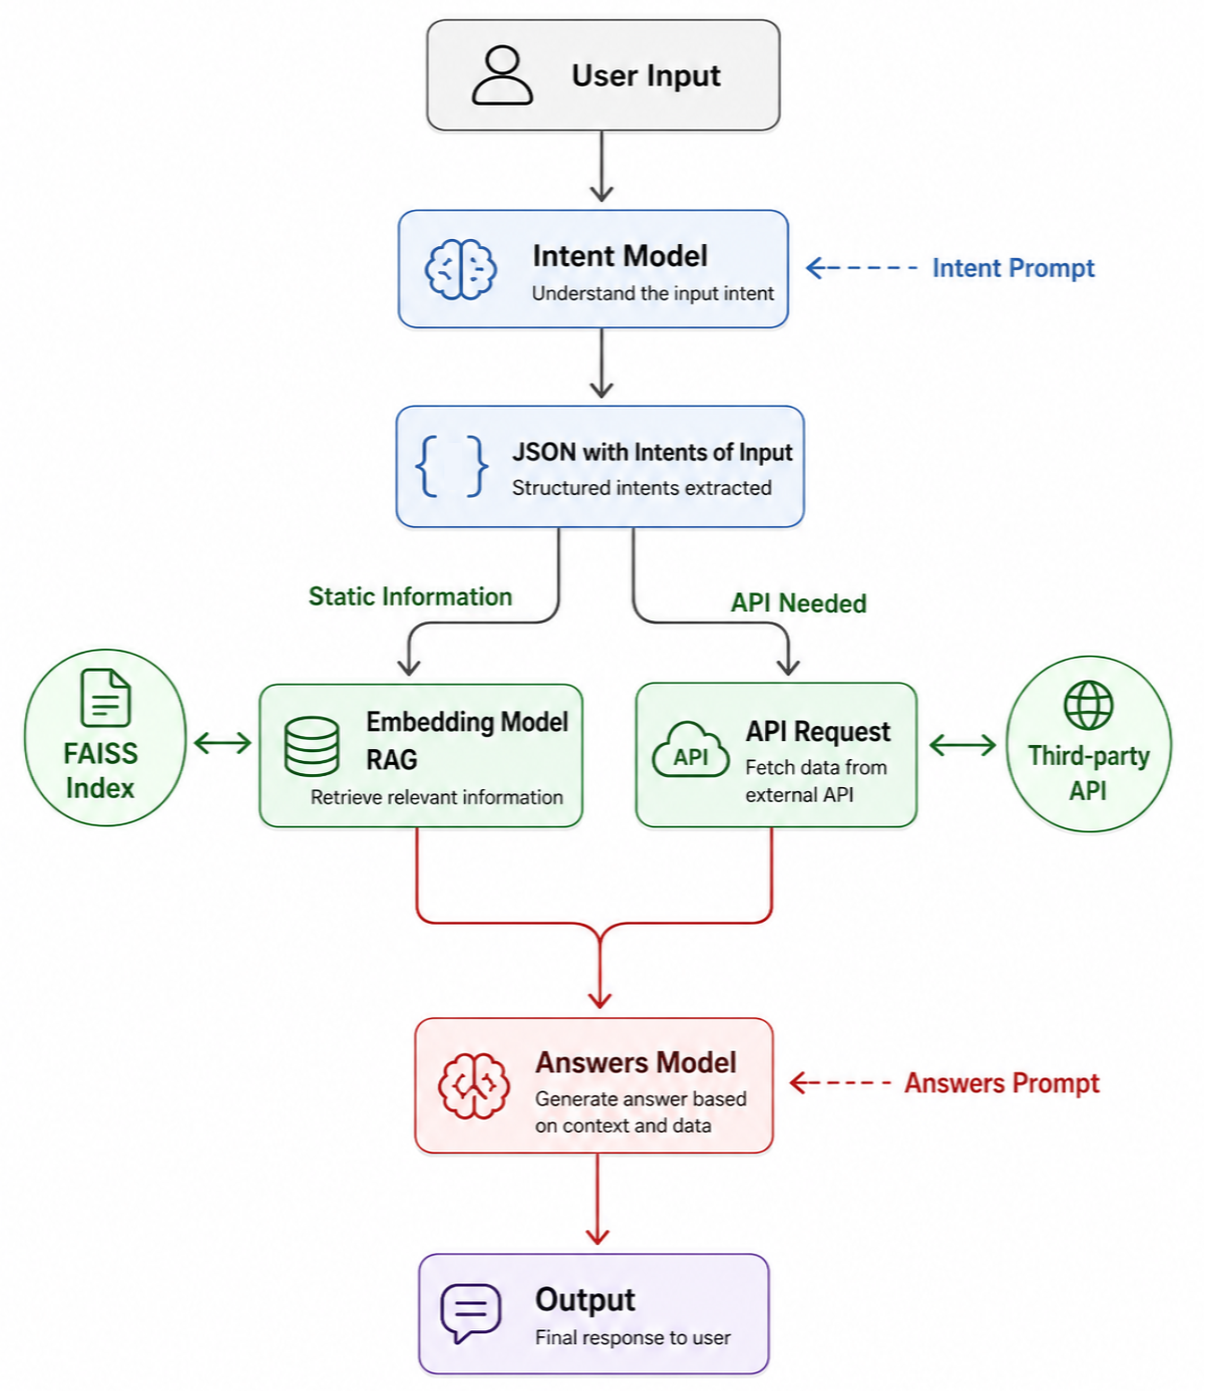
\includegraphics[width=1\linewidth]{fig/architecture.png}
    \caption{Pipeline architecture overview}
    \label{fig:architecture}
\end{figure}

\subsection*{Model Setup}
The system uses three specialized models:
\begin{itemize}
    \item \textbf{Intent Model:} Extracts structured information from user input, which determines whether static or live data is required, and outputs a JSON representation of the query. Specifically, \href{https://huggingface.co/mistralai/Mistral-7B-Instruct-v0.3}{Mistral-7B-Instruct-v0.3} is used. 
    \item \textbf{Embedding Model:} Encodes text into vector representations for similarity-based retrieval. \href{https://huggingface.co/sentence-transformers/paraphrase-multilingual-MiniLM-L12-v2}{Paraphrase-multilingual-MiniLM-L12-v2} is used, a sentence transformer model. 
    \item \textbf{Answer Model:} Generates the final natural language response based on the retrieved data, integrating all available information. It is the largest model in the pipeline, specifically \href{https://huggingface.co/Qwen/Qwen2.5-14B}{Qwen2.5-14B}.
\end{itemize}
This separation enables efficient processing, as smaller models handle intermediate steps, while a larger model is reserved for the generation of the final response.

\subsection*{Intent Extraction}
Initially, user input is processed by the intent model, guided by a comprehensive intent prompt, which specifies the model's role as well as the schema of the desired JSON output. Therefore, an intent decision table determines the conditions upon which an intent is identified, while additional constraints, rules and specific examples provide clear guidance to the model. The resulting file contains not only information on the detected intent, but also relevant parameters such as train number, departure and destination station, time information, as well as a measure of the model's confidence in answering the query accurately. \\
Valid intents that lead to an API request comprise \textbf{journey search}, \textbf{station timetable}, and \textbf{train status}. While the intent of \textbf{general info} aligns with the retrieval of static data and therefore sends a request to the RAG embedding model, there can also be \textbf{out of context} intents that are not supposed to be answered by the chatbot. 

\subsection*{Data Retrieval}
Depending on the extracted intent, the system retrieves the required information from either static or dynamic sources.

\subsubsection*{RAG}
Static knowledge is provided through a FAISS-based vector index built from the scraped websites listed in \ref{websites}. The data is split into chunks, embedded, and stored. At runtime, the user query is embedded and matched against the index to retrieve relevant context. The index is created once and reused, but automatically rebuilt when the embedding model changes. 

\subsubsection*{API Integration}
For dynamic information such as route planning or departure times, the system queries the \href{https://www.digitraffic.fi/en/railway-traffic/}{Digitraffic Railway Traffic API} through the structured JSON parameters constructed by the intent model. 

\subsection*{Answer Generation}
In addition to the data provided by either the RAG module or the API request, the answer model receives a static answer prompt that specifies its desired role and defines a list of rules it should follow. Examples for these rules include responding exclusively in natural, simple language and not inventing information that cannot be derived from the data gathered in the previous step. 

\subsection*{Implementation Structure}
The system is implemented as a modular Python codebase with a clear separation of concerns: \\ 
\textbf{Backend modules} handle API communication, configuration, and data processing. \\
\textbf{LLM engine modules} manage routing, model orchestration and configuration, as well as pipeline execution. \\
\textbf{Prompt files} define behavior for intent extraction and answer generation. \\
\textbf{Metadata} provides structured domain-specific information, such as a dictionary of all the train stations. \\ \\
Overall, the architecture combines structured intent processing with retrieval and generation techniques, enabling flexible handling of both static knowledge and real-time data, while remaining extensible for future improvements.

\section*{Evaluation and Results}
28 user queries were defined, each of them labeled with their correct intent, and provided to the chatbot system as test scenarios. The full set of queries including the complete output is documented in the Appendix.

\subsubsection*{Quantitative Evaluation}
The quantitative evaluation conducted is limited to intent extraction, i.e. whether the intent model was able to correctly identify the domain of the user query. The results are based on the 28 queries that represent different intents and are displayed in Table \ref{tab:quantitative}. \\
The findings show that intent was extracted with a high accuracy of 0.96, with train status demonstrating the only intent class where mistakes occurred during classification. More specifically, the recall value of 0.86 implies that one intended train status query was not identified as such. It is important to note that "other" was neglected due to the model trying to invent arbitrary information instead of correctly identifying that it is not supposed to have the necessary knowledge. Besides that, the intent classifier achieves a high overall performance. However, the evaluation results should be interpreted with caution due to the small dataset size (28 samples) and the absence of examples for the "other" class, which limits the generalizability of the findings. 

\begin{table}[h] 
\centering
\small
\caption{Intent Classification Performance}
\label{tab:quantitative}
\begin{tabular}{lcccc}
\toprule
\textbf{Class} & \textbf{Precision} & \textbf{Recall} & \textbf{F1-score} & \textbf{Support} \\
\midrule
general\_info       & 1.00 & 1.00 & 1.00 & 7 \\
journey\_search     & 1.00 & 1.00 & 1.00 & 7 \\
% other               & 0.00 & 0.00 & 0.00 & 0 \\
station\_timetable  & 1.00 & 1.00 & 1.00 & 7 \\
train\_status       & 1.00 & 0.86 & 0.92 & 7 \\
\midrule
\textbf{Accuracy}   & \multicolumn{4}{c}{0.96} \\
\midrule
% macro avg           & 0.80 & 0.77 & 0.78 & 28 \\
weighted avg        & 1.00 & 0.96 & 0.98 & 28 \\
\bottomrule
\end{tabular}
\end{table}

\subsubsection*{Qualitative Evaluation}
To assess whether the chatbot holds up with general-purpose LLMs in terms of accuracy and overall quality, responses to selected queries were compared against those of ChatGPT and Gemini. Due to the time-sensitive nature of transport data, the comparison focuses on qualitative aspects such as response structure, completeness, and grounding rather than factual correctness. \\
For journey search, timetable, and train status queries, the proposed system demonstrates clear advantages. By integrating external APIs, it provides precise and up-to-date information, including exact departure times and delay status. In contrast, general-purpose LLMs are unable to access real-time data and therefore produce generic or potentially outdated responses. \\
While the system performs well in scenarios where structured data is successfully retrieved and processed, several failure cases were observed during evaluation. In particular, the system occasionally produces the manually defined fallback response “I cannot answer the question with the provided data”, even when relevant information is available. This behavior indicates limitations in the answer generation stage, where the model does not fully utilize the provided context. These cases were observed multiple times within the evaluation dataset, suggesting a systematic issue rather than isolated errors, likely caused by an overly restrictive answer prompt. The latter was attempted to be refined several times, without any major breakthrough in achieving significantly more successful results. \\
For general information queries, both approaches perform well. However, LLMs tend to produce more fluent and user-friendly responses, while the chatbot system ensures correctness through retrieval from verified sources. \\
Overall, the results highlight a trade-off between linguistic quality and factual grounding. While general-purpose LLMs excel in natural language generation, the proposed system provides more reliable and domain-specific answers through the integration of structured data sources. An overview of the qualitative findings is displayed in Table \ref{tab:qualitative}.

\begin{table*}[t]
\centering
\caption{Qualitative Comparison of System Responses with ChatGPT and Gemini}
\label{tab:qualitative}
\begin{tabular}{p{3cm} p{4.5cm} p{4.5cm} p{4.5cm}}
\toprule
\textbf{Query Type} & \textbf{Proposed System} & \textbf{ChatGPT} & \textbf{Gemini} \\
\midrule

Journey Search &
Provides exact train, departure, arrival, and duration based on real-time API data. &
States travel is possible, gives typical duration, but no exact connection; refers to external tools. &
Similar to ChatGPT: general availability and duration, no real-time data, suggests checking official sources. \\

\midrule

Station Timetable &
Lists multiple departures with exact timestamps from API data. Detailed but slightly raw formatting. &
Describes frequent departures in general terms; no actual timetable provided. &
Gives general overview of departures; lacks specific times and real-time data. \\

\midrule

Train Status &
Confirms delay using real-time API data and current train location. &
Cannot access real-time data; advises checking official sources. &
Same limitation as ChatGPT; no real-time status available. \\

\midrule

General Information (RAG) &
Provides accurate, source-grounded rules (e.g., reservation required, restrictions on certain trains). &
Gives general rules about bike transport, but not operator-specific; may miss constraints. &
Similar to ChatGPT: generic explanation without guaranteed correctness. \\

\bottomrule
\end{tabular}
\end{table*}


% Tests with AI-Tool: 

% Query: "Hello, i want to go from Helsinki to Turku on Monday 4.5. in the morning. Which trains can I take?"

% \textbf{ChatGPT:} 
% Answer: Morning trains (approximate departures)
% ~05:25–05:30 → arrival ~07:30
% ~06:50–07:00 → arrival ~08:30–08:40
% ~08:30–08:40 → arrival ~10:35–10:40
% ~10:30–10:40 → arrival ~12:35–12:40

% → nearly all trains correct, but second one doesn't exist 
% → also a concrete service: InterCity train IC 41
% departs 06:53 from Helsinki
% arrives 08:34 in Turku
% → this is not a train from the official website 

% \textbf{Gemini:}
% Gives correct timetable, but one train in between is missing


% Follow up question: "I want to take the one at 08:30, can you tell me where exactly it stops and how much is a ticket?"
% \textbf{ChatGPT:} 
% → ChatGPT gives correct departure \& arrival times and also the correct stops in between 
% You also get a information about the ticket price from two different sources, but just a span and not the exact prices

% \textbf{Gemini:}
% → correct departure \& arrival times and correct stops
% → price range and also states additional fees for different classes or bicycle 


% Follow up question: "When i want to bring a bicycle, do I have to pay extra?" 
% → ChatGPT states correct information about regulations of taking a bicycle \& Gemini already gave this information in the answer before


% → ChatGPT \& Gemini can answer question regarding train connections, prices and regulations pretty precisely because it uses Online-Search


% Usage Scenarios:
% \begin{itemize}
%     \item I want to take a train from Helsinki to Tampere tomorrow around 8 am. What are my options?
%     \item Is my train IC 93 from 8:00 to 9:53 today on schedule?
%     \item How do I get from Tampere to Rovaniemi? (very long, indirect route)
%     \item I want to take train IC 93 tomorrow from 8:00 to 9:53. How much is the ticket?
%     \item I want to take a train from Helsinki to Tampere tomorrow at a flexible time. What's my cheapest option? 
%     \item Which cities can I reach from Kuopio without switching trains?
%     \item Which services does my train IC 93 at 8am today from Helsinki provide?
%     \item Was my train on schedule two months ago?
%     \item What trains are arriving to Oulo in the next hour?
% \end{itemize}

\section*{Limitations \& Future Work}
Despite the promising results, the chatbot exhibits several limitations that affect robustness and user experience.
\subsection*{Limitations}
A key limitation seems to be rooted in the answer generation component. In multiple cases, the system produces the aforementioned fallback response “I cannot answer the question with the provided data", even when the available data should suffice to give a response.  \\
Additionally, responses are sometimes too minimal or insufficiently processed. For example, timetable outputs may be unsorted or contain overly detailed timestamp syntax, and journey results may include only a single connection despite multiple available options. \\ 
The intent extraction component also introduces potential errors, as it does not always reliably produce the required JSON format, which can disrupt downstream processing. Moreover, for out-of-context user queries that go beyond the scope of the chatbot's capabilities, the intent model is unable to acknowledge its own limitation and instead produces hallucinated information. \\
Generally, the chatbot is not particularly robust and can easily fail to interpret user queries correctly, which also shows in the necessity to specify "Helsinki asema" instead of "Helsinki", for instance. \\
Furthermore, the system depends on external data sources, including APIs and a limited set of scraped websites, which may affect coverage and reliability. Finally, the evaluation is based on a small dataset (28 queries) and focuses on qualitative aspects due to the time-sensitive domain.

\subsection*{Future Work}
Future improvements should primarily focus on the answer prompt and response strategy, ensuring that the model consistently utilizes available data and avoids unnecessary fallback responses. \\
Enhancing response quality and formatting would improve usability, for example by sorting timetables, simplifying timestamps, and presenting multiple relevant options. \\
The intent model can be improved through better prompt design, stricter output validation, and a larger evaluation dataset. Expanding the RAG pipeline with additional data sources would further improve coverage for general queries. \\
Finally, future work could include larger-scale evaluation and user studies to better assess system performance and usability.

\section*{Conclusion}
This work presented a modular chatbot system for Finnish railway transportation that combines intent extraction, retrieval-augmented generation, and external API integration to answer user queries. The system is capable of handling multiple query types, including journey search, station timetables, train status, and general informational requests. \\
The evaluation demonstrates that integrating structured data sources provides a clear advantage over general-purpose language models in time-sensitive scenarios. The system is able to generate precise and up-to-date responses by leveraging real-time API data and verified information from retrieved documents. In contrast, general-purpose models produce more fluent but often generic or non-actionable responses in such contexts. \\
At the same time, the results highlight several limitations. In particular, the answer generation component does not always make effective use of available data, leading to unnecessary fallback responses. Additionally, the overall response quality can be improved in terms of formatting, completeness, and usability. These findings emphasize that system performance is not only determined by model capability, but also by prompt design and integration logic. \\
In conclusion, the proposed approach demonstrates that combining language models with external data sources is a promising strategy for building reliable domain-specific assistants. Future improvements should focus on enhancing response generation, increasing robustness in intent handling, and expanding the underlying data sources to further improve coverage and user experience.

% By now the following was implemented:
% \begin{itemize}
%     \item complete Pipeline: Query → intent extraction → RAG / API → build prompt → LLM answer generator 
%     \item API Request handler that can get all informations about train schedules and delays (works)
%     \item RAG handler that scrapes websites with embedding and a faiss index (doesn't work yet on arnes) 
% \end{itemize}

% What we will work on: 
% \begin{itemize}
%     \item integrate RAG into pipeline and test it on the cluster
%     \item try different models and compare results
%     \item try different prompt mechanism (more friendly, more fact-based)
    
% \end{itemize}

%----------------------------------------------------------------------------------------
%	REFERENCE LIST
%----------------------------------------------------------------------------------------
\bibliographystyle{unsrt}
\bibliography{report}

\clearpage
\appendix
\section*{Evaluation Logs}
\label{app:logs}

\lstinputlisting[breaklines=true]{pipeline_log.txt}

\end{document}

